

\hypertarget{v-results}{%
\subsection{V results}\label{v-results}}

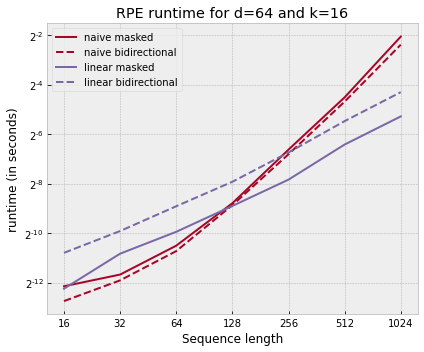
\includegraphics{images/timings/runtimes_RPE.png}

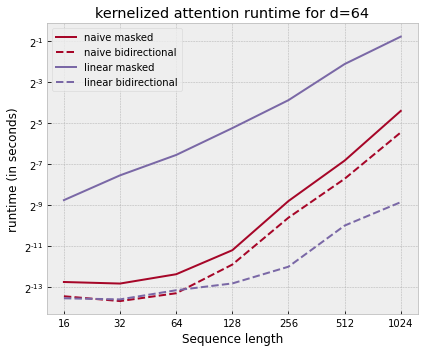
\includegraphics{images/timings/runtimes_KA.png}

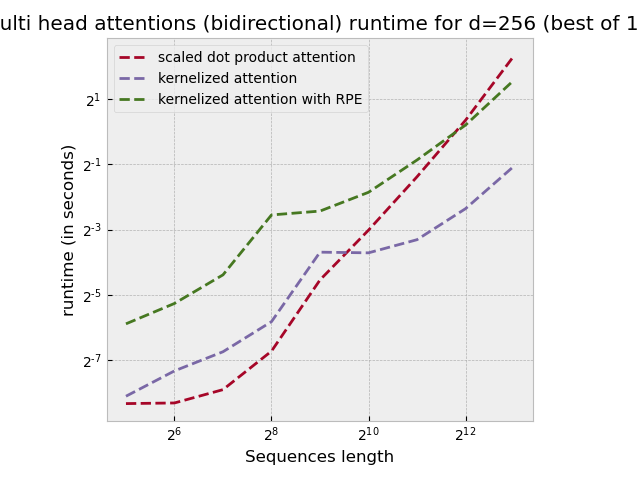
\includegraphics{images/timings/runtimes_MHA.png}

\hypertarget{conclusion}{%
\subsection{Conclusion}\label{conclusion}}

In the present work an easily implemented algorithm to compute
\href{https://arxiv.org/abs/1803.02155}{Shaw et al.~(2018)}'s relative
positional embedding with linear complexity has been presented. An
implementation of \href{https://arxiv.org/abs/2009.14794}{Choromanski et
al.~(2020)}'s prefix sum algorithm that doesn't requires custom CUDA
code (while maintaining linear complexity) was also presented.

These two elements allowed to define a kernelized attention function
with relative positional encoding, that can be computed with linear
complexity with regards to sequence length. The proposed model presents
linear scalability with sequence length, can be implemented out of the
boxe in neural network framework, and is adapted to sequence to sequence
problems instead of being restricted to encoders only models.
